\documentclass{article}

\usepackage{polski}
\usepackage{graphicx}
\usepackage{float}
\usepackage[T1]{fontenc}
\usepackage[polish]{babel}
\usepackage[utf8]{inputenc}
\usepackage{lmodern}
\selectlanguage{polish}

\author{Anna Pływaczyk, 200340}
\title{Przeszukiwanie grafu w \LaTeX-u }
\date{28.05.2014}
\begin{document}
\maketitle

\section{Wstęp}
Graf jest strukturą matematyczną służącą do przedstawienia relacji między obiektami. W uproszczeniu graf to zbiór wierzchołków, które mogą być połączone dowolnymi krawędziami. 
\newline
Przeszukiwanie grafu to czynność polegająca na odwiedzeniu w jakiś usystematyzowany sposób wszystkich wierzchołków grafu w celu zebrania potrzebnych informacji.  
\newline
Celem ćwiczenia jest zaimplementowanie grafu oraz 3 różnych poszukiwań drogi między wierzchołkami:
\begin{itemize}
\item BFS - Breadth-first search
\item DFS - Depth-first search
\item A* - A-star
\end{itemize}
Następnie należało przetestować szybkość przeszukiwań.
 
\section{Rodzaje przeszukiwań grafu}
\subsection{BFS - Breadth-first search}
BFS inaczej zwane przeszukiwanie wszerz wykorzystuje strukturę danych zwaną kolejką. Przechodzenie rozpoczyna od zadanego wierzchołka i polega na odwiedzeniu wszystkich osiągalnych z niego wierzchołków. Wykorzystywany do odnajdowania najkrótszej drogi w grafie. 
\subsection{DFS - Depth-first search}
DFS inaczej zwane przeszukiwanie w głąb wykorzystuje strukturę danych zwaną stosem. Rozpoczyna działanie w wybranym wierzchołku. Następnie przechodzi wzdłuż dostępnej krawędzi do sąsiada tego wierzchołka, który nie został jeszcze odwiedzony. Przechodzenie trwa do momentu aż zostanie osiągnięty wierzchołek nie posiadający sąsiadów. Wtedy procedura wraca do poprzednio odwiedzonego wierzchołka i kontynuuje działanie wzdłuż dostępnej krawędzi.
\subsection{A* - A-star}
A-star jest algorytmem heurystycznym znajdowania najkrótszej ścieżki w grafie ważonym  z dowolnego wierzchołka do wierzchołka spełniającego określony warunek zwany testem celu. Algorytm jest zupełny i optymalny, oznacza to iż znajduje ścieżkę jeżeli tylko taka istnieje i przy tym ta ścieżka jest najkrótsza. 
 
\section{Porównanie przeszukiwań}
\begin{figure}[h]
	\centering
	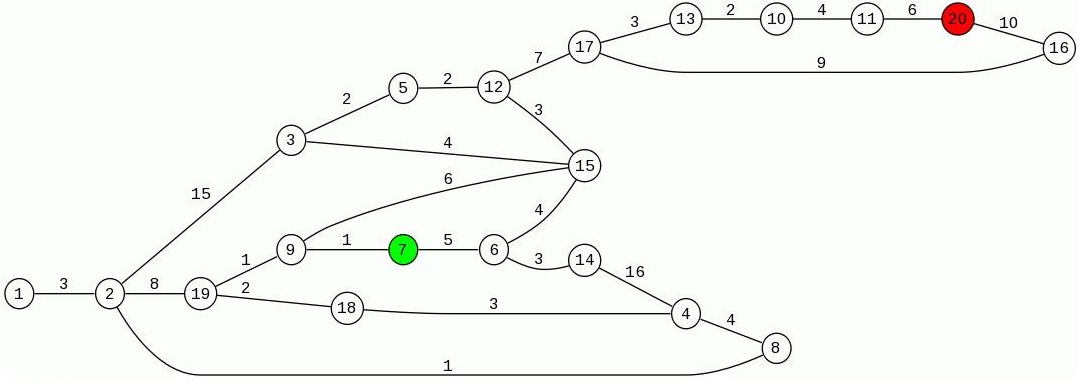
\includegraphics[scale=0.5]{grafik.jpg}
	\caption{Graf, który został przetestowany. Wierzchołek zielony oznacza start, czerwony - meta.}
	\end{figure}
	\newpage
	
	\begin{table}
	\caption{Porównanie szybkości przeszukiwań grafu.}
	\begin{center}
	\begin{tabular}{|c||l||l||l|}
	\hline  & BFS & DFS & A* \\ \hline 
	odwiedzone wierzchołki & 26 & 19 & 16 \\ \hline
	droga po wierzchołkach & 7,6,15,12,17,16,20 & 7,9,15,12,17,16,20 & 7,6,15,12,17,13,10,11,20 \\ \hline
	długość drogi & 38 & 36 & 34 \\ \hline
	\end{tabular}
	\end{center}		 
	\end{table}
\section{Wnioski}
Najszybsze poszukiwanie drogi uzyskamy za pomocą algorytmu A*. Zarówno liczba odwiedzonych wierzchołków jak droga do pokonania jest najkrótsza, pomimo że ilość wierzchołków w wyznaczonej drodze jest większa niż w pozostałych algorytmach.
\newline
Algorytmy BFS i DFS wyznaczają drogę zawierającą mniej wierzchołków niż A-star jednak liczba odwiedzonych wierzchołków i droga jest zdecydowanie większa. Spośród tych dwóch poszukiwań szybszy jest BFS.
\newline
Zdecydowanie jeżeli potrzebujemy najkrótszej i najszybszej ścieżki powinniśmy używać A*.

\end{document}
